% Options for packages loaded elsewhere
\PassOptionsToPackage{unicode}{hyperref}
\PassOptionsToPackage{hyphens}{url}
\PassOptionsToPackage{dvipsnames,svgnames,x11names}{xcolor}
%
\documentclass[
  letterpaper,
  DIV=11,
  numbers=noendperiod]{scrartcl}

\usepackage{amsmath,amssymb}
\usepackage{iftex}
\ifPDFTeX
  \usepackage[T1]{fontenc}
  \usepackage[utf8]{inputenc}
  \usepackage{textcomp} % provide euro and other symbols
\else % if luatex or xetex
  \usepackage{unicode-math}
  \defaultfontfeatures{Scale=MatchLowercase}
  \defaultfontfeatures[\rmfamily]{Ligatures=TeX,Scale=1}
\fi
\usepackage{lmodern}
\ifPDFTeX\else  
    % xetex/luatex font selection
  \setmainfont[]{Inter}
  \setsansfont[]{Inter}
  \setmathfont[]{Fira Math}
\fi
% Use upquote if available, for straight quotes in verbatim environments
\IfFileExists{upquote.sty}{\usepackage{upquote}}{}
\IfFileExists{microtype.sty}{% use microtype if available
  \usepackage[]{microtype}
  \UseMicrotypeSet[protrusion]{basicmath} % disable protrusion for tt fonts
}{}
\makeatletter
\@ifundefined{KOMAClassName}{% if non-KOMA class
  \IfFileExists{parskip.sty}{%
    \usepackage{parskip}
  }{% else
    \setlength{\parindent}{0pt}
    \setlength{\parskip}{6pt plus 2pt minus 1pt}}
}{% if KOMA class
  \KOMAoptions{parskip=half}}
\makeatother
\usepackage{xcolor}
\setlength{\emergencystretch}{3em} % prevent overfull lines
\setcounter{secnumdepth}{5}
% Make \paragraph and \subparagraph free-standing
\ifx\paragraph\undefined\else
  \let\oldparagraph\paragraph
  \renewcommand{\paragraph}[1]{\oldparagraph{#1}\mbox{}}
\fi
\ifx\subparagraph\undefined\else
  \let\oldsubparagraph\subparagraph
  \renewcommand{\subparagraph}[1]{\oldsubparagraph{#1}\mbox{}}
\fi


\providecommand{\tightlist}{%
  \setlength{\itemsep}{0pt}\setlength{\parskip}{0pt}}\usepackage{longtable,booktabs,array}
\usepackage{calc} % for calculating minipage widths
% Correct order of tables after \paragraph or \subparagraph
\usepackage{etoolbox}
\makeatletter
\patchcmd\longtable{\par}{\if@noskipsec\mbox{}\fi\par}{}{}
\makeatother
% Allow footnotes in longtable head/foot
\IfFileExists{footnotehyper.sty}{\usepackage{footnotehyper}}{\usepackage{footnote}}
\makesavenoteenv{longtable}
\usepackage{graphicx}
\makeatletter
\def\maxwidth{\ifdim\Gin@nat@width>\linewidth\linewidth\else\Gin@nat@width\fi}
\def\maxheight{\ifdim\Gin@nat@height>\textheight\textheight\else\Gin@nat@height\fi}
\makeatother
% Scale images if necessary, so that they will not overflow the page
% margins by default, and it is still possible to overwrite the defaults
% using explicit options in \includegraphics[width, height, ...]{}
\setkeys{Gin}{width=\maxwidth,height=\maxheight,keepaspectratio}
% Set default figure placement to htbp
\makeatletter
\def\fps@figure{htbp}
\makeatother

\usepackage{amsmath, xparse}
\usepackage{fancyvrb, fvextra}
\usepackage{unicode-math}
\usepackage{svg}
\usepackage{multicol}
\usepackage{listings}
\usepackage{systeme}
\usepackage{xifthen}
\DefineVerbatimEnvironment{Highlighting}{Verbatim}{breaklines,commandchars=\\\{\}}
\lstset{basicstyle=\ttfamily\footnotesize,breaklines=true}
\newcommand\rowop[1]{\scriptstyle\smash{\xrightarrow[\vphantom{#1}]{\mkern-4mu#1\mkern-4mu}}}
\DeclareDocumentCommand\converttorows%
{>{\SplitList{,}}m}%
{\ProcessList{#1}{\converttorow}}
\NewDocumentCommand{\converttorow}{m}
{\ifthenelse{\isempty{#1}}{}{\rowop{#1}}\\}

\DeclareDocumentCommand \rowops{m}
{\;
\begin{matrix}
\converttorows {#1}
\end{matrix}
\; }
\KOMAoption{captions}{tableheading}
\makeatletter
\@ifpackageloaded{caption}{}{\usepackage{caption}}
\AtBeginDocument{%
\ifdefined\contentsname
  \renewcommand*\contentsname{Table of contents}
\else
  \newcommand\contentsname{Table of contents}
\fi
\ifdefined\listfigurename
  \renewcommand*\listfigurename{List of Figures}
\else
  \newcommand\listfigurename{List of Figures}
\fi
\ifdefined\listtablename
  \renewcommand*\listtablename{List of Tables}
\else
  \newcommand\listtablename{List of Tables}
\fi
\ifdefined\figurename
  \renewcommand*\figurename{Figure}
\else
  \newcommand\figurename{Figure}
\fi
\ifdefined\tablename
  \renewcommand*\tablename{Table}
\else
  \newcommand\tablename{Table}
\fi
}
\@ifpackageloaded{float}{}{\usepackage{float}}
\floatstyle{ruled}
\@ifundefined{c@chapter}{\newfloat{codelisting}{h}{lop}}{\newfloat{codelisting}{h}{lop}[chapter]}
\floatname{codelisting}{Listing}
\newcommand*\listoflistings{\listof{codelisting}{List of Listings}}
\makeatother
\makeatletter
\makeatother
\makeatletter
\@ifpackageloaded{caption}{}{\usepackage{caption}}
\@ifpackageloaded{subcaption}{}{\usepackage{subcaption}}
\makeatother
\ifLuaTeX
  \usepackage{selnolig}  % disable illegal ligatures
\fi
\usepackage{bookmark}

\IfFileExists{xurl.sty}{\usepackage{xurl}}{} % add URL line breaks if available
\urlstyle{same} % disable monospaced font for URLs
\hypersetup{
  colorlinks=true,
  linkcolor={blue},
  filecolor={Maroon},
  citecolor={Blue},
  urlcolor={Blue},
  pdfcreator={LaTeX via pandoc}}

\author{}
\date{}

\begin{document}

\begin{titlepage}

    \newcommand{\HRule}{\rule{\linewidth}{0.5mm}}
    
    \center
    
    \vspace{10cm}

    \textsc{\LARGE Gwinnett School of Math, Science, and Technology }\\[0.3cm]
    
    \vspace{0.5cm}

    \HRule \\[0.4cm]
    { \huge \bfseries Macroeconomics Yearlong Notes}\\[0.03cm]
    \HRule \\[1.5cm]
    
    \begin{minipage}{0.4\textwidth}
    \begin{flushleft} \Large
    Anish Goyal \\1st Period
    \end{flushleft}
    \end{minipage}
    ~
    \begin{minipage}{0.4\textwidth}
    \begin{flushright} \Large
    Michael Burbine\\Educator
    \end{flushright}
    \end{minipage}\\[1cm]
    
    {\huge 2023-2024}\\[1cm]
    
    
\includegraphics{img/logo.png}\\
    \vfill
    \end{titlepage}

\newpage

\renewcommand*\contentsname{Table of Contents}
{
\hypersetup{linkcolor=}
\setcounter{tocdepth}{4}
\tableofcontents
}
\newpage{}

\section{Types of Goods (01/08)}\label{types-of-goods-0108}

\subsection{Characteristics of the Four Types of
Goods}\label{characteristics-of-the-four-types-of-goods}

\begin{itemize}
\tightlist
\item
  \textbf{Rivalrous} goods are those that can only be consumed by one
  person at a time.
\item
  \textbf{Non-rivalrous} goods are those that can be consumed by
  multiple people at the same time.
\item
  \textbf{Excludable} goods are those that can be restricted to certain
  people.
\item
  \textbf{Non-excludable} goods are those that cannot be restricted to
  certain people.
\item
  If a public good is overcrowded enough, it can become a common
  resource
\end{itemize}

\subsection{The Four Types of Goods}\label{the-four-types-of-goods}

\begin{longtable}[]{@{}
  >{\raggedright\arraybackslash}p{(\columnwidth - 4\tabcolsep) * \real{0.1707}}
  >{\raggedright\arraybackslash}p{(\columnwidth - 4\tabcolsep) * \real{0.5041}}
  >{\raggedright\arraybackslash}p{(\columnwidth - 4\tabcolsep) * \real{0.3171}}@{}}
\toprule\noalign{}
\begin{minipage}[b]{\linewidth}\raggedright
\end{minipage} & \begin{minipage}[b]{\linewidth}\raggedright
\textbf{Non-rivalrous}
\end{minipage} & \begin{minipage}[b]{\linewidth}\raggedright
\textbf{Rivalrous}
\end{minipage} \\
\midrule\noalign{}
\endhead
\bottomrule\noalign{}
\endlastfoot
\textbf{Non-excludable} & \begin{minipage}[t]{\linewidth}\raggedright
\begin{verbatim}
                  *Public Goods*\
          (e.g. Sunset, Common Knowledge)
\end{verbatim}
\end{minipage} & \begin{minipage}[t]{\linewidth}\raggedright
\emph{Common-Pool/Common Resources}\\
(e.g.~Irrigation Systems, Libraries)\strut
\end{minipage} \\
\textbf{Excludable} & \begin{minipage}[t]{\linewidth}\raggedright
\emph{(Toll/Club/Artificially Scarce) Goods/Natural monopolies}\\
(e.g.~Day-Care Centers, Country Clubs)\strut
\end{minipage} & \begin{minipage}[t]{\linewidth}\raggedright
\emph{Private Goods}\\
(e.g.~Donuts, Personal Computers)\strut
\end{minipage} \\
\end{longtable}

\subsection{Examples}\label{examples}

\begin{verbatim}
              Case Scenario                   | Type of Good/Service
\end{verbatim}

------------------------------------------------- \textbar{}
-------------------- A college education \textbar{} Artificially scarce
A manicure or pedicure \textbar{} Private good Stone Mountain park
\textbar{} Artificially scarce State park campgrounds \textbar{}
Artificially scarce National defense \textbar{} Public good Peach Pass
lane on I-85 \textbar{} Artificially scarce Fish in the ocean \textbar{}
Common resource Street lights \textbar{} Public good Netflix/Hulu
\textbar{} Artificially scarce Flu shot \textbar{} Private good Tornado
safety shelter \textbar{} Public good Bottled water in a tornado safety
shelter \textbar{} Common resource Hearing a tornado siren \textbar{}
Public good Going to an almost empty public beach \textbar{} Public good
Going to an overcrowded public beach \textbar{} Common resource
St.~Lawrence SeaWay \textbar{} Natural monopoly Flying on a commercial
airplane \textbar{} Natural monopoly Flying a single seat private
airplane \textbar{} Private good Wedding guests eating a slice of the
wedding-cake \textbar{} Common resource Cake sold at a bakery \textbar{}
Private good

\newpage{}

\section{Introduction to Externalities
(01/09-01/10)}\label{introduction-to-externalities-0109-0110}

\subsection{Overview}\label{overview}

\begin{itemize}
\tightlist
\item
  An \textbf{externality} is a cost/benefit that affects a \emph{third
  party} who did not choose to incur that cost/benefit.
\item
  They are a type of \textbf{market failure} because they are \emph{not}
  accounted for in the price of the good/service.
\item
  The deadweight loss (DWL) of positive externalities will point to the
  right and vice-versa for negative externalities.

  \begin{itemize}
  \tightlist
  \item
    Which means the DWL triangle always points to the social optimum
    quantity.
  \end{itemize}
\end{itemize}

\subsection{\texorpdfstring{Internalizing an Externality (aka \emph{how
to fix an
externality})}{Internalizing an Externality (aka how to fix an externality)}}\label{internalizing-an-externality-aka-how-to-fix-an-externality}

\subsubsection{Problems with
externalities}\label{problems-with-externalities}

\begin{enumerate}
\def\labelenumi{\arabic{enumi})}
\tightlist
\item
  Private individuals won't take into account the external
  costs/benefits
\item
  Public goods and common pool resources tend to lack property rights
\end{enumerate}

\subsubsection{Coase Theorem (the fix!)}\label{coase-theorem-the-fix}

``We can fix externalities without the government if we\ldots{}''

\begin{enumerate}
\def\labelenumi{\arabic{enumi})}
\tightlist
\item
  Give property rights to people
\item
  Minimize transaction costs
\end{enumerate}

\subsubsection{Examples}\label{examples-1}

Methods the government can employ to internalize an externality in a
free market:

\begin{itemize}
\tightlist
\item
  Pollution or emission limits
\item
  ``Pollution credits'' for private firms to buy and sell in the market
\end{itemize}

\newpage{}

\subsection{Positive Externality in
Consumption}\label{positive-externality-in-consumption}

\begin{figure}[H]

{\centering 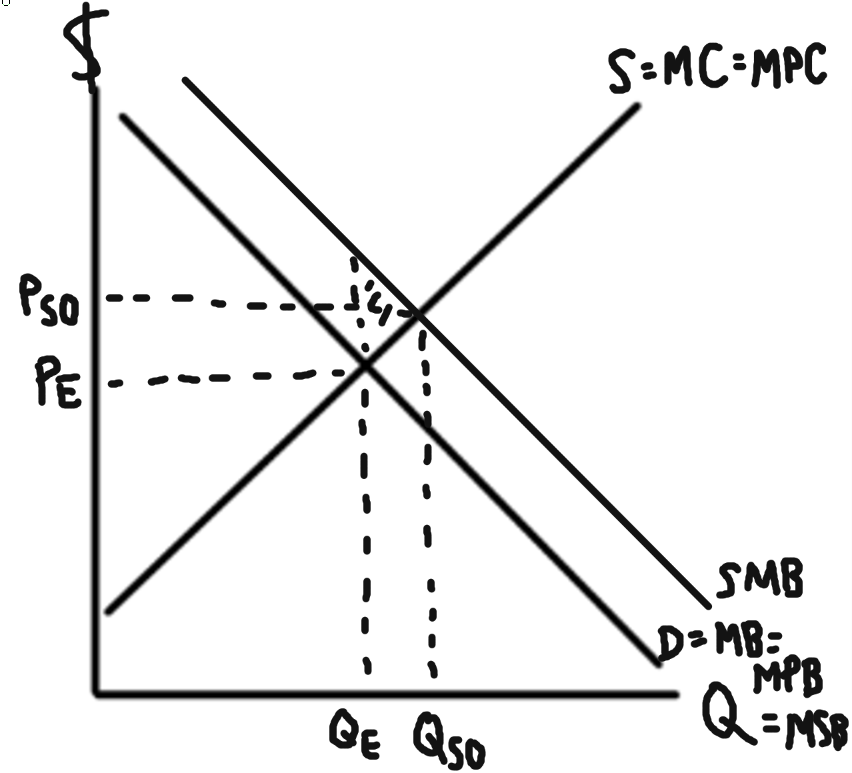
\includegraphics[width=0.5\textwidth,height=\textheight]{img/pos-cons.png}

}

\caption{Positive Externality in Consumption}

\end{figure}%

\subsubsection{Examples}\label{examples-2}

\begin{itemize}
\tightlist
\item
  Consumption of education
\item
  Consumption of health care
\item
  Advertisement can lead to an increase of demand in the free market
  \(\therefore MPB\) goes up and moves the market toward \(MSB\).
\end{itemize}

\subsubsection{Spillover Effect}\label{spillover-effect}

\begin{itemize}
\tightlist
\item
  The spillover effect is \(MEB = MSB-MPB\).
\item
  \(MPB < MSB\)
\item
  \(MPC = MSC\)
\end{itemize}

\subsubsection{Internalizing the Spillover
Effect}\label{internalizing-the-spillover-effect}

\begin{itemize}
\tightlist
\item
  The external \textbf{benefits} can be internalized by
  \textbf{subsidizing} the product/service to the consumers of the
  good/service.
\item
  The government intervention will move the private market to
  \textbf{social optimum} where \(MSB = MSC\).
\end{itemize}

\newpage{}

\subsection{Negative Externality in
Consumption}\label{negative-externality-in-consumption}

\begin{figure}[H]

{\centering 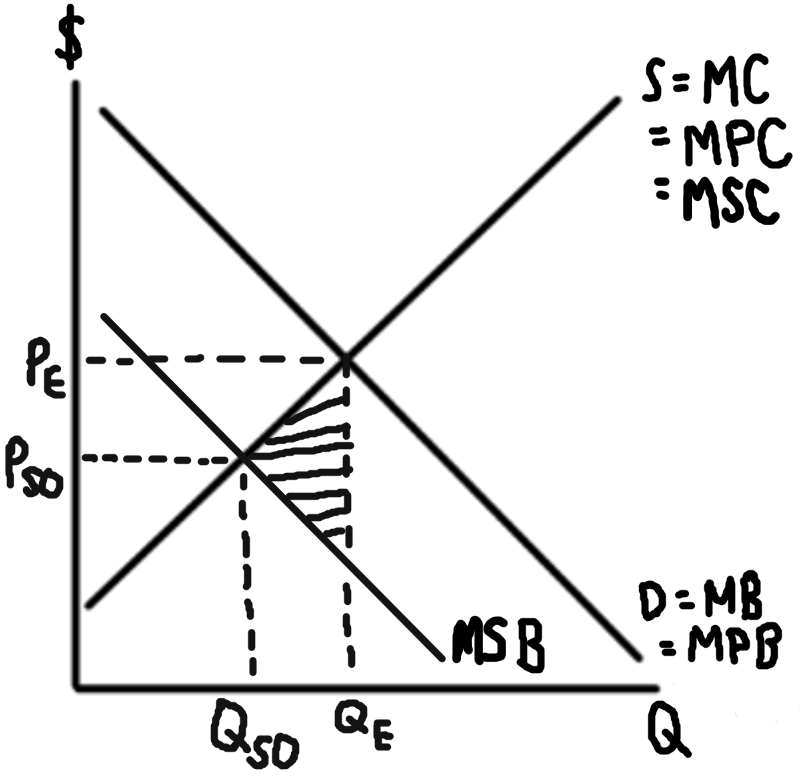
\includegraphics[width=0.45\textwidth,height=\textheight]{img/neg-cons.png}

}

\caption{Negative Externality in Consumption}

\end{figure}%

\subsubsection{Examples}\label{examples-3}

\begin{itemize}
\tightlist
\item
  Smoking in public/passive smoking
\item
  Pollution due to fossil fuels
\item
  Playing loud music
\item
  Discarding garbage in public places
\end{itemize}

\subsubsection{Spillover Effect}\label{spillover-effect-1}

\begin{itemize}
\tightlist
\item
  The spillover effect is \(MEB = MSB-MPB\).
\item
  \(MPB > MSB\)
\item
  \(MPC = MSC\)
\end{itemize}

\subsubsection{Internalizing the Spillover
Effect}\label{internalizing-the-spillover-effect-1}

\begin{itemize}
\tightlist
\item
  The external \textbf{benefits} can be internalized by \textbf{imposing
  a tax} on the product/service to the consumers of the good/service.
\item
  The government intervention will move the private market to
  \textbf{social optimum} where \(MSB = MSC\).
\end{itemize}

\newpage{}

\subsection{Positive Externality in
Production}\label{positive-externality-in-production}

\begin{figure}[H]

{\centering 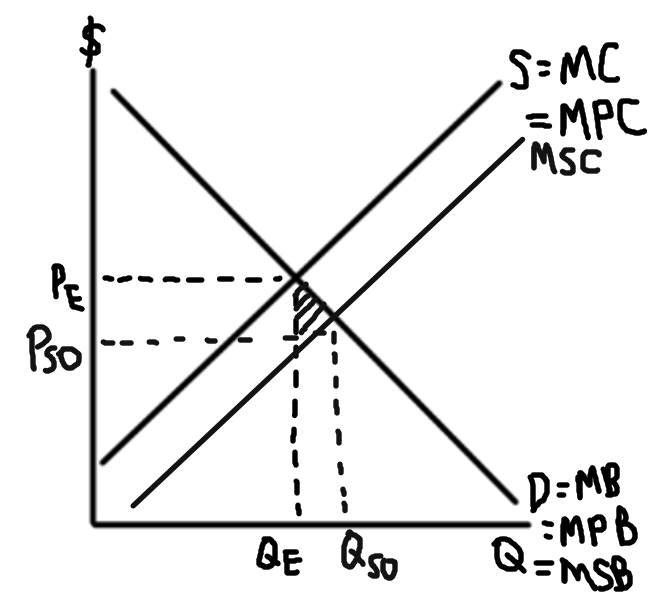
\includegraphics[width=0.5\textwidth,height=\textheight]{img/pos-prod.png}

}

\caption{Positive Externality in Production}

\end{figure}%

\subsubsection{Examples}\label{examples-4}

\begin{itemize}
\tightlist
\item
  Companies invest in training/professional development of their
  employees.
\item
  Firms invest in research and development (R\&D).
\end{itemize}

\subsubsection{Spillover Effect}\label{spillover-effect-2}

\begin{itemize}
\tightlist
\item
  The spillover effect is \(MEC = MSC-MPC\).
\item
  \(MPB = MSB\)
\item
  \(MPC > MSC\)
\end{itemize}

\subsubsection{Internalizing the Spillover
Effect}\label{internalizing-the-spillover-effect-2}

\begin{itemize}
\tightlist
\item
  The external \textbf{costs} can be internalized by
  \textbf{subsidizing} the product/service to the producers of the
  good/service.
\item
  The government intervention will move the private market to
  \textbf{social optimum} where \(MSB = MSC\).
\end{itemize}

\newpage{}

\subsection{Negative Externality in
Production}\label{negative-externality-in-production}

\begin{figure}[H]

{\centering 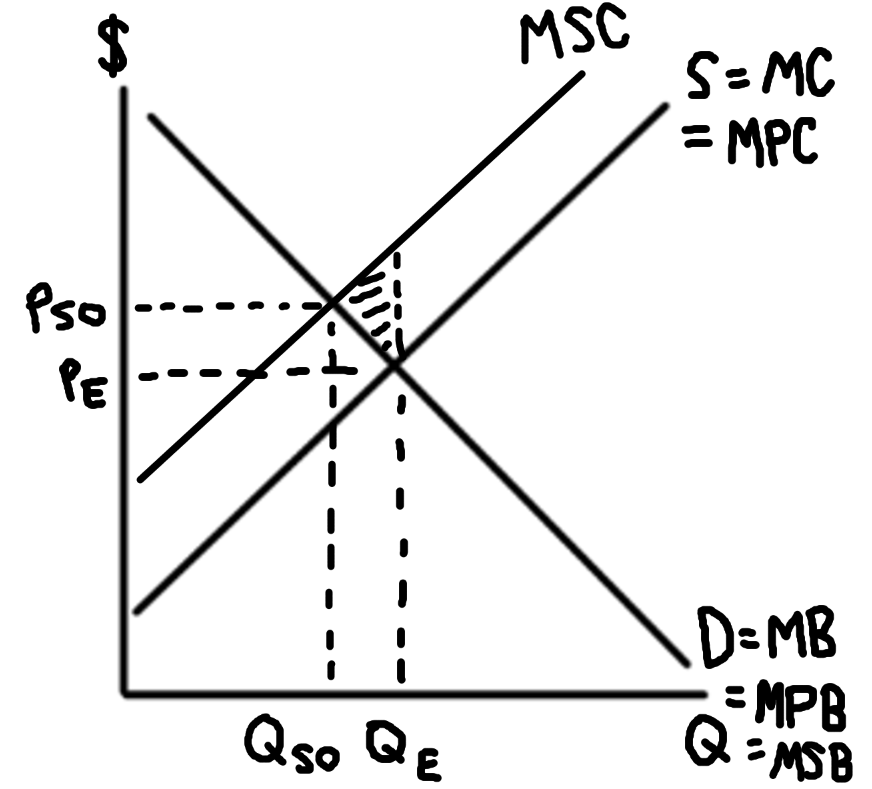
\includegraphics[width=0.5\textwidth,height=\textheight]{img/neg-prod.png}

}

\caption{Negative Externality in Production}

\end{figure}%

\subsubsection{Examples}\label{examples-5}

\begin{itemize}
\tightlist
\item
  Firms produce chemicals that cause pollution \(\therefore\) local
  fisherman cannot catch fish.
\item
  Construction of roads lead to change of landscape and parks
\item
  Coal fired power plants
\end{itemize}

\subsubsection{Spillover Effect}\label{spillover-effect-3}

\begin{itemize}
\tightlist
\item
  The spillover effect is \(MEC = MSC-MPC\).
\item
  \(MPB = MSB\)
\item
  \(MPC < MSC\)
\end{itemize}

\subsubsection{Internalizing the Spillover
Effect}\label{internalizing-the-spillover-effect-3}

\begin{itemize}
\tightlist
\item
  The external \textbf{costs} can be internalized by \textbf{imposing a
  tax} on the product/service to the producers of the good/service.
\item
  The government intervention will move the private market to
  \textbf{social optimum} where \(MSB = MSC\).
\end{itemize}

\newpage{}

\section{Income Inequality (01/12)}\label{income-inequality-0112}

\subsection{The Lorenz Curve and Gini
Coefficient}\label{the-lorenz-curve-and-gini-coefficient}

\begin{itemize}
\tightlist
\item
  The \textbf{Lorenz Curve} \(L(x)\) is a graphical representation of
  the distribution of income in a country.

  \begin{itemize}
  \tightlist
  \item
    The x-axis is the cumulative percentage of the population
    (0\%-100\%).
  \item
    The y-axis is the cumulative percentage of income (0\%-100\%).
  \item
    It is always accompanied by the line \(y=x\) which represents
    \textbf{perfect equality}.
  \end{itemize}
\item
  The \textbf{Gini Coefficient} \(G\) is a numerical representation of
  the Lorenz Curve.

  \begin{itemize}
  \tightlist
  \item
    It is the ratio of the area between the Lorenz Curve and the line
    \(y=x\) to the area under the line \(y=x\).

    \begin{itemize}
    \tightlist
    \item
      \(G = \frac{A}{A+B}\) where
      \(A = \int_{0}^{1} \left[x-L(x)\right] \ \mathrm{d}x\) and
      \(B = \int_{0}^{1}L(x) \ \mathrm{d}x\).
    \end{itemize}
  \item
    The closer \(G\) is to 1, the more unequal the distribution of
    income is.
  \end{itemize}
\end{itemize}

\begin{figure}[H]

{\centering 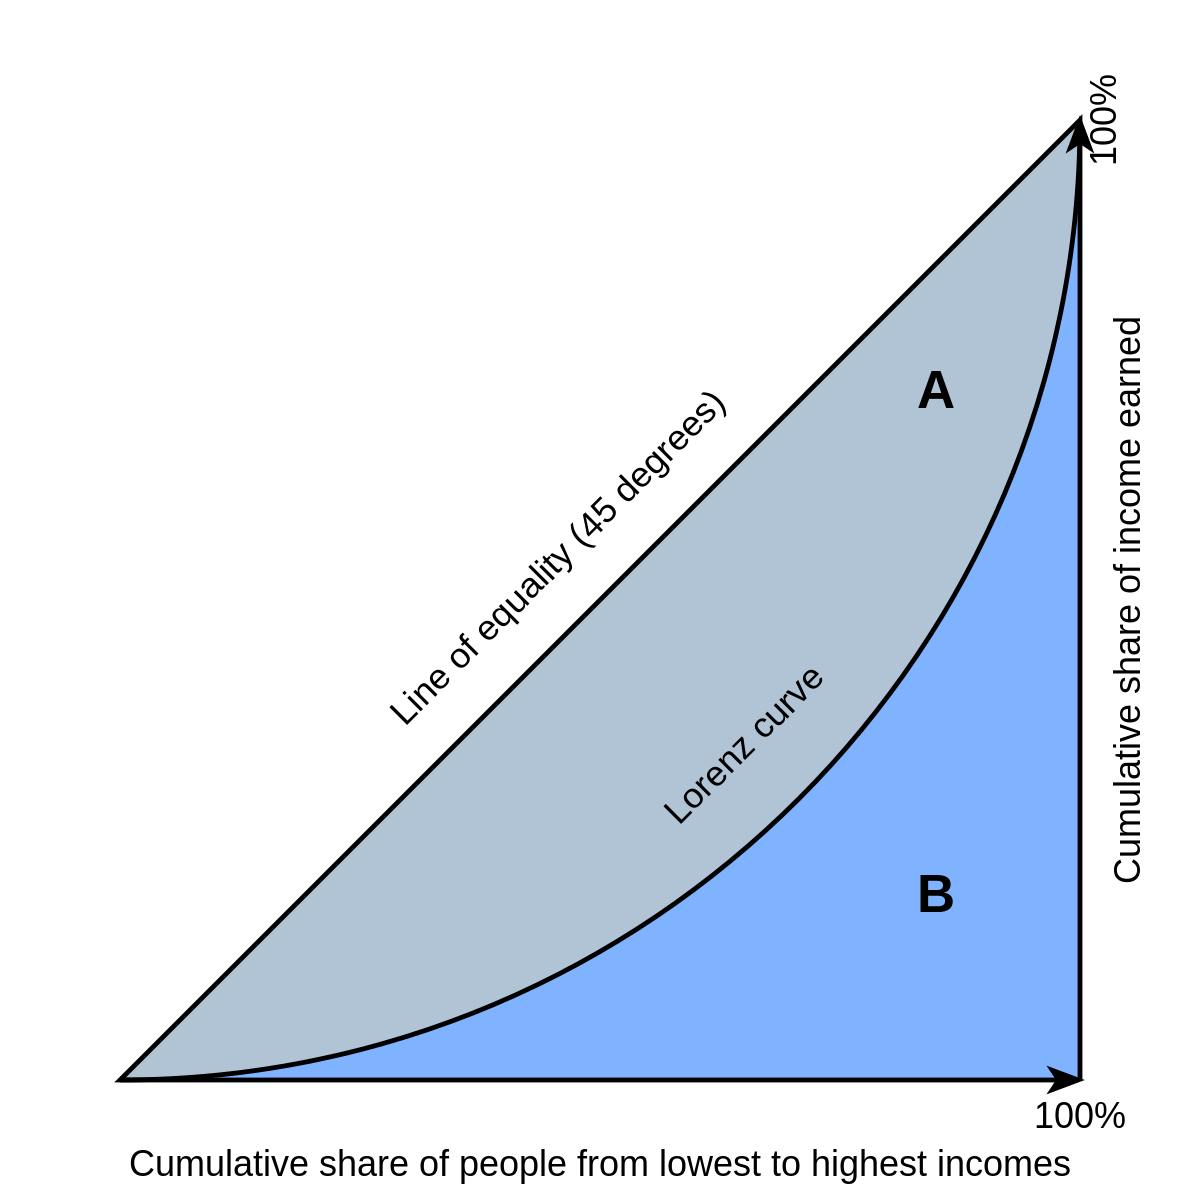
\includegraphics[width=0.68\textwidth,height=\textheight]{img/lorenz.png}

}

\caption{Visual depiction of the Lorenz Curve}

\end{figure}%

As demonstrated in \emph{Figure 6} below:

\begin{itemize}
\tightlist
\item
  If \(G\) is 0, then the Lorenz Curve is \textbf{also} the line \(y=x\)
  because the area between both curves \(A\) is 0.
\item
  If \(G\) is 1, then the Lorenz Curve is the x-axis (\(y=0\)) because
  \(A+B\) must also equal the area under \(y=x\), or \(\frac{1}{2}\).
\end{itemize}

\begin{figure}[H]

{\centering 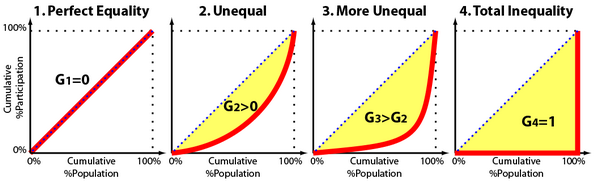
\includegraphics[width=1\textwidth,height=\textheight]{img/varying-gini.png}

}

\caption{Varying Gini Coefficients and their corresponding Lorenz
Curves}

\end{figure}%

\subsection{Deriving Simpler Expressions for the Gini
Coefficient}\label{deriving-simpler-expressions-for-the-gini-coefficient}

Since we know that
\(A+B = \int_{0}^{1} x \ \mathrm{d}x = \left.\frac{x^2}{2}\right\vert_{0}^{1} = \frac{1}{2}\),
we can derive ``easier'' expressions to calculate the Gini Coefficient
\(G\).

\subsubsection{\texorpdfstring{Deriving
\(G=2A\)}{Deriving G=2A}}\label{deriving-g2a}

\begin{align}
G &= \frac{A}{A+B}\tag{Initial Gini Coefficient formula} \\
\frac{1}{G} &= \frac{A+B}{A}\tag{Reciprocate} \\
\frac{A}{G} &= A+B\tag{Multiply by $A$} \\
\frac{A}{G}-A &= B\tag{Subtract $A$}
\end{align}

\newpage{}

Now we can substitute \(B\) into the original area formula:

\begin{align}
A + B &= \frac{1}{2}\tag{Area under $y=x$} \\
A+\left(\frac{A}{G}-A\right) &= \frac{1}{2}\tag{Substitute $B$} \\
\frac{A}{G} &= \frac{1}{2}\tag{Simplify} \\
\cfrac{A}{\frac{1}{2}} &= G\tag{Simplify} \\
2A &= G\tag{Multiply by 2}
\end{align}

\subsubsection{\texorpdfstring{Deriving
\(G=1-2B\)}{Deriving G=1-2B}}\label{deriving-g1-2b}

Since we've already expressed \(B\) in terms of \(A\), we just need to
get \(A\) in terms of \(B\).

\begin{align}
G = 2A \tag{Previous derivation} \\
\frac{G}{2} = A \tag{Divide by 2} \\
\frac{G}{2} = \frac{1}{2}-B\tag{Substitute $A$ using the expression $A=\frac{1}{2}-B$} \\
G = 1-2B\tag{Multiply by 2}
\end{align}

Therefore, two \textbf{alternate expressions} for the Gini Coefficient
are:

\begin{align}
G &= 2A \\
G &= 1-2B
\end{align}

\newpage{}

\subsection{Negative Externalities: Public vs.~Private Resolution and
More on the Coase Theorem
(01/16)}\label{negative-externalities-public-vs.-private-resolution-and-more-on-the-coase-theorem-0116}

\subsubsection{Conditions}\label{conditions}

Recall that the \textbf{Coase Theorem} states market failures will
always be resolved by the free market. Here are all the conditions for
Coase Theorem to hold true:

\begin{itemize}
\tightlist
\item
  Both sides are rational and willing to negotiate to maximize their own
  utility.
\item
  Low to no transaction costs
\item
  Private property rights are well-defined
\item
  Perfect information is available to both sides and they have the same
  leverage
\end{itemize}

\subsubsection{Miscellaneous Market
Failures}\label{miscellaneous-market-failures}

There are a couple of other market failures that the government should
try to combat, based on the types of markets we learned about \emph{in
previous units}:

\begin{itemize}
\tightlist
\item
  \textbf{Monopoly}: A single firm controls the entire market.

  \begin{itemize}
  \tightlist
  \item
    This will cause the firm to produce \emph{less} than the social
    optimum and still charge a \emph{greater price}.
  \end{itemize}
\item
  \textbf{Monopsony}: A single firm controls the entire labor market.

  \begin{itemize}
  \tightlist
  \item
    This will cause the firm to hire \emph{less} than optimum and for a
    \emph{lower wage}.
  \end{itemize}
\end{itemize}

\section{Intro to Macronomic Indicators
(01/22-01/23)}\label{intro-to-macronomic-indicators-0122-0123}

GDP stands for Gross Domestic Product. These three words are important
to understand:

\begin{itemize}
\tightlist
\item
  Gross: Not just profits - \emph{total} value
\item
  Domestic: Made WITHIN the borders of the US
\item
  Products: Goods and services which have been produced
\end{itemize}

Formal definition of GDP: ~ \textbf{GDP} is: the sum of the market value
of all final goods and services produced within the United States in a
given time period (usually a year).

\newpage{}

\begin{longtable}[]{@{}
  >{\raggedright\arraybackslash}p{(\columnwidth - 4\tabcolsep) * \real{0.1143}}
  >{\raggedright\arraybackslash}p{(\columnwidth - 4\tabcolsep) * \real{0.4857}}
  >{\raggedright\arraybackslash}p{(\columnwidth - 4\tabcolsep) * \real{0.4000}}@{}}
\toprule\noalign{}
\begin{minipage}[b]{\linewidth}\raggedright
Concept
\end{minipage} & \begin{minipage}[b]{\linewidth}\raggedright
Is
\end{minipage} & \begin{minipage}[b]{\linewidth}\raggedright
Is NOT
\end{minipage} \\
\midrule\noalign{}
\endhead
\bottomrule\noalign{}
\endlastfoot
Sum & TOTAL & Single industry or market \\
Value & Based on the market price of the goods and services &
subjective \\
Final & new and complete goods and services; ready for use &
intermediate goods/services; used goods \\
G\&S & ONLY a good or service & FINANCIAL ASSETS
(Stock/Bonds/ETFs/Crypto) \\
Produced & MADE & transfer payments or foreign aid \\
Domestically & WITHIN US borders & US citizens abroad \\
Time & This year (NEW production) & OLD G\&S, Goodwill \\
\end{longtable}

\subsection{Calculating GDP}\label{calculating-gdp}

GDP is known as tam easure of \emph{national income accounting}. What
are the two accounting techniques used in measuring GDP?

\begin{itemize}
\tightlist
\item
  \textbf{Expenditure Approach}: Measures GDP by adding up all the
  spending on final goods and services produced in the nation during the
  year.

  \begin{itemize}
  \tightlist
  \item
    \(GDP = C + I + G + (X-M)\); C=Consumption, I=Investment,
    G=Government Spending, X=Exports, M=Imports
  \end{itemize}
\item
  \textbf{Income Approach}: Measures GDP by adding up all the income
  earned by the factors of production (land, labor, capital,
  entrepreneurship) during the year.

  \begin{itemize}
  \tightlist
  \item
    \(GDP = W + I + R + P\); W=Wages, I=Interest, R=Rents, P=Profits
  \end{itemize}
\item
  Therefore, \(GDP = C + I + G + (X-M) = W + I + R + P\)
\end{itemize}

\newpage{}

\subsection{Circular Flow Model and
Leakages}\label{circular-flow-model-and-leakages}

\begin{figure}[H]

{\centering 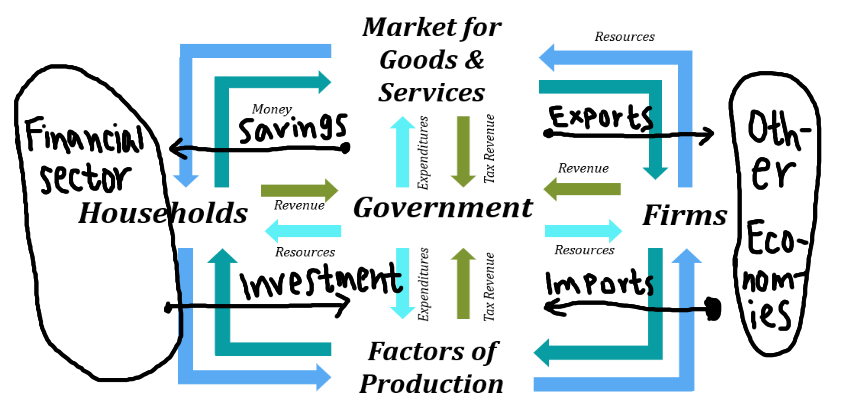
\includegraphics[width=0.75\textwidth,height=\textheight]{img/circular-flow.png}

}

\caption{Circular Flow Model}

\end{figure}%

\begin{itemize}
\tightlist
\item
  \textbf{Leakages} are the non-consumption uses of income, such as
  savings, taxes, and imports.
\item
  Your piggy bank and transfer payments are leakages.
\end{itemize}

\subsection{Gross National Product}\label{gross-national-product}

\begin{itemize}
\tightlist
\item
  \textbf{GNP} is the sum of the value of all final goods and services
  prodced by Americans anywhere in the world during a time period.
\end{itemize}

\subsection{Examples of Factors that Affect
GDP}\label{examples-of-factors-that-affect-gdp}

\subsubsection{Which of these is Counted in
GDP?}\label{which-of-these-is-counted-in-gdp}

\begin{itemize}
\tightlist
\item
  A monthly check received by an economics student who has been granted
  a government scholarship.
\item
  A farmer's purchase of a new tractor \(\checkmark\)
\item
  A plumber's purchase of a two-year-old used truck \(\times\)
\item
  Cashing a U.S. government bond \(\times\)
\item
  The services of a mechanic in fixing the radiator in his own car
\item
  A Social Security check from the government to a retired store clerk
\item
  An increase in business inventories \(\checkmark\)
\item
  The government's purchase of a new submarine for the Navy
  \(\checkmark\)
\item
  A barber's income from cutting hair \(\checkmark\)
\item
  Income received from the sale of Nike Stock \(\times\)
\end{itemize}

\subsubsection{Which of these is counted in GDP and part of
consumption?}\label{which-of-these-is-counted-in-gdp-and-part-of-consumption}

\begin{itemize}
\tightlist
\item
  You Spend \$7 at the movies \(\checkmark\)
\item
  A family pays a contractor \$200k for a house he built them this year
  \(\times\)
\item
  A family pays \$75k for a house built three years ago \(\times\)
\item
  An accountant pays a tailor \$175 to sew a suit for her \(\checkmark\)
\item
  The government increases its defense expenditures by \$1 billion
  \(\times\)
\item
  The government makes a \$300 Social Security payment to a retired
  person \(\times\)
\item
  You buy General Motors Corp.~stock for \$1k in the stock market
  \(\times\)
\item
  At the end of the year, a flour-milling firm finds that its
  inventories of grain and flour are \$10k above the amounts of its
  inventories at the beginning of the year \(\times\)
\item
  A homemaker works hard caring for her spouse and two children
  \(\times\)
\item
  Ford Motor Co.~buys new auto-making robots \(\times\)
\item
  You pay \$300 a month to rent an apartment \(\checkmark\)
\item
  Apple Computers builds a new factory in the US \(\times\)
\item
  RJ Reynolds Co.~buys control of Nabisco \(\times\)
\item
  You buy a new Toyota that was made in Japan. \(\times\)
\item
  You pay tuition to attend college. \(\checkmark\)
\end{itemize}

\subsubsection{Which of these is Counted in GDP and part of
investment?}\label{which-of-these-is-counted-in-gdp-and-part-of-investment}

\begin{itemize}
\tightlist
\item
  A family pays a contractor \$200k for a house he built them this year
  \(\checkmark\)
\item
  A family pays \$75k for a house built three years ago \(\times\)
\item
  The government increases its defense expenditures by \$1 billion
  \(\times\)
\item
  The government makes a \$300 Social Security payment to a retired
  person \(\times\)
\item
  You buy General Motors Corp.~stock for \$1k in the stock market
  \(\times\)
\item
  At the end of the year, a flour-milling firm finds that its
  inventories of grain and flour are \$10k above the amounts of its
  inventories at the beginning of the year \(\checkmark\)
\item
  A homemaker works hard caring for her spouse and two children
  \(\times\)
\item
  Ford Motor Co.~buys new auto-making robots \(\checkmark\) \(\times\)
\item
  Apple Computers builds a new factory in the US \(\checkmark\)
\item
  RJ Reynolds Co.~buys control of Nabisco \(\times\)
\item
  You buy a new Toyota that was made in Japan. \(\times\)
\end{itemize}

\subsubsection{Which of these is Counted in GDP and part of government
spending?}\label{which-of-these-is-counted-in-gdp-and-part-of-government-spending}

\begin{itemize}
\tightlist
\item
  A family pays \$75k for a house built three years ago \(\times\)
\item
  The government increases its defense expenditures by \$1 billion
  \(\checkmark\)
\item
  The government makes a \$300 Social Security payment to a retired
  person \(\times\)
\item
  You buy General Motors Corp.~stock for \$1k in the stock market
  \(\times\)
\item
  A homemaker works hard caring for her spouse and two children
  \(\times\)
\item
  RJ Reynolds Co.~buys control of Nabisco \(\times\)
\item
  You buy a new Toyota that was made in Japan. \(\times\)
\end{itemize}

\subsubsection{Which of these is Counted in GDP and part of net
export/import?}\label{which-of-these-is-counted-in-gdp-and-part-of-net-exportimport}

\begin{itemize}
\tightlist
\item
  A family pays \$75k for a house built three years ago \(\times\)
\item
  The government makes a \$300 Social Security payment to a retired
  person \(\times\)
\item
  You buy General Motors Corp.~stock for \$1k in the stock market
  \(\times\)
\item
  A homemaker works hard caring for her spouse and two children
  \(\times\)
\item
  RJ Reynolds Co.~buys control of Nabisco \(\times\)
\item
  You buy a new Toyota that was made in Japan. \(\checkmark\)
\end{itemize}

\subsubsection{We count only the final price of a good or service in
GDP.
Why?}\label{we-count-only-the-final-price-of-a-good-or-service-in-gdp.-why}

We don't count intermediate and used goods/services because then we
would be \textbf{double-counting}; also, the good/service in question
might have not been made in the time period analyzed if it wasn't final.

\subsubsection{A purely financial transaction will not be counted in
GDP.
Why?}\label{a-purely-financial-transaction-will-not-be-counted-in-gdp.-why}

Because a purely financial transaction doesn't involve consumption,
investment, government spending, exports, or imports.

\subsubsection{When a home-owner does home-improvement work, the labor
is not counted in GDP.
Why?}\label{when-a-home-owner-does-home-improvement-work-the-labor-is-not-counted-in-gdp.-why}

They're not paying themself or making any profits off of their work to
contribute to the income approach for calculating GDP.

\subsection{Calculating GDP Examples}\label{calculating-gdp-examples}

\subsubsection{Example 1}\label{example-1}

Suppose that personal income is \$500 billion, personal taxes are \$100
billion, and depreciation is \$50 billion. Disposable income is equal to
which of the following?

\(DI = PT - PT = 100 - 50 = \$50 \text{ billion}\)

\subsubsection{My Practice}\label{my-practice}

Suppose that personal income is \$100 billion, personal taxes are \$50
billion, and depreciation is \$25 billion. Disposable income is equal to
which of the following?

\subsubsection{Example 2}\label{example-2}

\begin{longtable}[]{@{}
  >{\raggedright\arraybackslash}p{(\columnwidth - 2\tabcolsep) * \real{0.4167}}
  >{\raggedright\arraybackslash}p{(\columnwidth - 2\tabcolsep) * \real{0.2083}}@{}}
\toprule\noalign{}
\endhead
\bottomrule\noalign{}
\endlastfoot
Wages & \$50 Billion \\
Rent & \$20 Billion \\
Private Investment Spending & \$10 Billion \\
Exports & \$30 Billion \\
Interest Payments & \$40 Billion \\
HH Profit & \$80 Billion \\
\end{longtable}

What is the GDP?
\(GDP = W + R + I + X + P = 50 + 20 + 10 + 30 + 80 = \$190 \text{ billion}\)

\subsubsection{My Practice}\label{my-practice-1}

\begin{longtable}[]{@{}
  >{\raggedright\arraybackslash}p{(\columnwidth - 2\tabcolsep) * \real{0.4167}}
  >{\raggedright\arraybackslash}p{(\columnwidth - 2\tabcolsep) * \real{0.2222}}@{}}
\toprule\noalign{}
\endhead
\bottomrule\noalign{}
\endlastfoot
Wages & \$90 Billion \\
Rent & \$40 Billion \\
Private Investment Spending & \$10 Billion \\
Corporate Taxes & \$50 Billion \\
Interest Payments & \$100 Billion \\
HH Profit & \$90 Billion \\
\end{longtable}

What is the GDP?
\(GDP = W + R + I + X + P = 90 + 40 + 10 + 0 + 90 = \$230 \text{ billion}\)

\subsubsection{Example 3}\label{example-3}

\begin{longtable}[]{@{}
  >{\raggedright\arraybackslash}p{(\columnwidth - 2\tabcolsep) * \real{0.4167}}
  >{\raggedright\arraybackslash}p{(\columnwidth - 2\tabcolsep) * \real{0.2083}}@{}}
\toprule\noalign{}
\endhead
\bottomrule\noalign{}
\endlastfoot
Consumption Spending & \$50 Billion \\
Individual Income Taxes & \$20 Billion \\
Private Investment Spending & \$10 Billion \\
Corporate Taxes & \$20 Billion \\
Exports & \$30 Billion \\
Imports & \$40 Billion \\
Government Purchases & \$80 Billion \\
\end{longtable}

What is the GDP?

\subsubsection{My Practice}\label{my-practice-2}

\begin{longtable}[]{@{}
  >{\raggedright\arraybackslash}p{(\columnwidth - 2\tabcolsep) * \real{0.4167}}
  >{\raggedright\arraybackslash}p{(\columnwidth - 2\tabcolsep) * \real{0.2222}}@{}}
\toprule\noalign{}
\endhead
\bottomrule\noalign{}
\endlastfoot
Consumption Spending & \$70 Billion \\
State Income Taxes & \$10 Billion \\
Private Investment Spending & \$50 Billion \\
Corporate Taxes & \$80 Billion \\
Net Exports & -\$40 Billion \\
Government Purchases & \$50 Billion \\
\end{longtable}

What is the GDP?

Using the prior table and the expenditure approach, what percent of GDP
is comprised of consumption, investment, and government spending?

How is this possible?

If a firm experiences depreciation of factor resources, which component
of GDP is negatively affected?

\subsubsection{Example 4}\label{example-4}

\begin{longtable}[]{@{}
  >{\raggedright\arraybackslash}p{(\columnwidth - 2\tabcolsep) * \real{0.3333}}
  >{\raggedright\arraybackslash}p{(\columnwidth - 2\tabcolsep) * \real{0.2639}}@{}}
\toprule\noalign{}
\endhead
\bottomrule\noalign{}
\endlastfoot
Aggregate Data & Value (Billions) \\
Consumption Spending & 10 \\
Employee Compensation & 7 \\
Government Spending & 60 \\
Interest Payments & 10 \\
Net Exports & -50 \\
Profits & 5 \\
Rents & 5 \\
Savings & 10 \\
\end{longtable}

Calculate GDP using both approaches.

Do both approaches yield equal GDP values? Why or why not?

\subsubsection{My Practice}\label{my-practice-3}

\begin{longtable}[]{@{}
  >{\raggedright\arraybackslash}p{(\columnwidth - 2\tabcolsep) * \real{0.3333}}
  >{\raggedright\arraybackslash}p{(\columnwidth - 2\tabcolsep) * \real{0.2639}}@{}}
\toprule\noalign{}
\endhead
\bottomrule\noalign{}
\endlastfoot
Aggregate Data & Value (Billions) \\
Consumption Spending & 190 \\
Employee Compensation & 200 \\
Government Spending & 100 \\
Interest Payments & 100 \\
Investment Spending & 90 \\
Net Exports & 60 \\
Profits & 50 \\
Rents & 50 \\
Savings & 50 \\
\end{longtable}

Calculate GDP using both approaches.

Do both approaches yield equal GDP values? Why or why not?

\subsubsection{Example 5}\label{example-5}

A country consists of 2 firms. Firm A's total revenue is \$200 million.
The cost of their inputs is \$50 million. Firm B's total revenue is
\$100 million. The cost of their inputs is \$10 million. What is the
total value added in this economy?

\subsubsection{My Practice}\label{my-practice-4}

\begin{longtable}[]{@{}
  >{\raggedright\arraybackslash}p{(\columnwidth - 6\tabcolsep) * \real{0.3472}}
  >{\raggedright\arraybackslash}p{(\columnwidth - 6\tabcolsep) * \real{0.1250}}
  >{\raggedright\arraybackslash}p{(\columnwidth - 6\tabcolsep) * \real{0.1250}}
  >{\raggedright\arraybackslash}p{(\columnwidth - 6\tabcolsep) * \real{0.1250}}@{}}
\toprule\noalign{}
\endhead
\bottomrule\noalign{}
\endlastfoot
Kingdom of Burbonia & Firm A & Firm B & Firm C \\
Firm's Sales & 20 & 50 & 100 \\
\begin{minipage}[t]{\linewidth}\raggedright
Cost of Intermediate\\
Goods Purchased by\\
Each firm\strut
\end{minipage} & \begin{minipage}[t]{\linewidth}\raggedright
10\\
\strut \\
\strut
\end{minipage} & \begin{minipage}[t]{\linewidth}\raggedright
40\\
\strut \\
\strut
\end{minipage} & \begin{minipage}[t]{\linewidth}\raggedright
40\\
\strut \\
\strut
\end{minipage} \\
\end{longtable}

What is the total value added in the Kingdom of Burbonia, measured in
millions of dollars?

\subsubsection{Challenge Problem}\label{challenge-problem}

Consumption is one third of total GDP. Gross Private Investment Spending
and Government Spending, Combined, are equal to consumption spending.
Exports are twice the number of imports. Imports are \$50 million.
Government spending is four times as much as investment.

What is consumption spending?

What is investment spending?

What is government spending?

What are exports?

What is GDP?

\newpage{}

\section{Advanced GDP Calculations
(01/25)}\label{advanced-gdp-calculations-0125}

\subsection{NGDP vs.~RGDP}\label{ngdp-vs.-rgdp}

\subsubsection{If we want to measure the amount of production using
current prices, what economic measure should we
use?}\label{if-we-want-to-measure-the-amount-of-production-using-current-prices-what-economic-measure-should-we-use}

Nominal GDP

\subsubsection{If we want to measure the amount of production using base
year prices, what economic measure should we
use?}\label{if-we-want-to-measure-the-amount-of-production-using-base-year-prices-what-economic-measure-should-we-use}

Real GDP

\subsubsection{Define ``REAL''}\label{define-real}

Accounting for inflation by referencing some initial level of price.

\subsubsection{What does RGDP show?}\label{what-does-rgdp-show}

The measure of true product, accounting for inflation

\subsubsection{What are the formulas for types of
GDP?}\label{what-are-the-formulas-for-types-of-gdp}

\begin{longtable}[]{@{}cc@{}}
\toprule\noalign{}
Nominal GDP & Real GDP \\
\midrule\noalign{}
\endhead
\bottomrule\noalign{}
\endlastfoot
\(\Sigma (Q_c \cdot P_c)\) & \(\Sigma (Q_c \cdot P_{c,\text{base}})\) \\
\end{longtable}

\subsubsection{Growth rate (percent change)
formula:}\label{growth-rate-percent-change-formula}

\(\frac{\text{New GDP}-\text{Old GDP}}{\text{Old GDP}} \cdot 100\%\)

For the base year, the RGDP always equals the NGDP.

\subsubsection{Standard of living}\label{standard-of-living}

\begin{itemize}
\tightlist
\item
  We use RGDP to measure the standard of living because it accounts for
  inflation.
\item
  RGDP per capita is the best measure of standard of living.
\end{itemize}

\subsubsection{Inflation/Deflation}\label{inflationdeflation}

\begin{itemize}
\tightlist
\item
  \(\frac{NGDP}{RGDP} \cdot 100\%\) is the deflator value (\(DF\)).
\item
  If \(DF > 100\%\) (\(NGDP > RGDP\)), there is inflation.
\item
  If \(DF < 100\%\) (\(NGDP < RGDP\)), there is deflation.
\item
  If \(DF = 100\%\) (\(NGDP = RGDP\)), prices are staying the same.
\item
  Disinflation is when the rate of inflation is decreasing, but
  inflation is still occurring nonetheless.
\item
  The deflator is always 100\% in the base year.
\end{itemize}

\subsubsection{What limitations does GDP have as an economic
measure?}\label{what-limitations-does-gdp-have-as-an-economic-measure}

\begin{itemize}
\tightlist
\item
  It doesn't account for non-market production (e.g.~stay-at-home
  parents)
\item
  It doesn't account for the underground economy (e.g.~drug dealers)
\item
  It doesn't account for negative externalities (e.g.~pollution)
\end{itemize}

\section{Unemployment (01/29)}\label{unemployment-0129}

\subsection{Questions on introductory unemployment
terms}\label{questions-on-introductory-unemployment-terms}

\begin{enumerate}
\def\labelenumi{\arabic{enumi}.}
\tightlist
\item
  Who constitutes as being employed?
\end{enumerate}

If they worked full or part time during the past week or is on vacation
or sick leave from a regular job.

\begin{enumerate}
\def\labelenumi{\arabic{enumi}.}
\setcounter{enumi}{1}
\tightlist
\item
  Who constitutes as being unemployed?
\end{enumerate}

If they did not work during the preceding week but made some effort to
find work in the past four weeks.

\begin{enumerate}
\def\labelenumi{\arabic{enumi}.}
\setcounter{enumi}{2}
\tightlist
\item
  Who constitutes as being out of the labor force?
\end{enumerate}

People who are not employed and haven't looked for a job in four weeks.
Institutionalized (prison), military, and those younger than 16 as well.
Discouraged workers, full time students, unpaid homemakers, and retirees
are examples.

\begin{enumerate}
\def\labelenumi{\arabic{enumi}.}
\setcounter{enumi}{3}
\tightlist
\item
  Who constitutes a discouraged worker? Do they cause an underestimate
  or overestimate of the unemployment rate?
\end{enumerate}

Workers tha thave given up looking ofr a job, now considered out of the
labor force.

\begin{enumerate}
\def\labelenumi{\arabic{enumi}.}
\setcounter{enumi}{4}
\tightlist
\item
  Is the entire population considered for unemployment calculations?
\end{enumerate}

Only adults (16+), non-institutionalized, civilian, nonretired
population.

\subsection{Types of unemployment}\label{types-of-unemployment}

\textbf{Frictional unemployment}

\begin{itemize}
\tightlist
\item
  Unemployment that is initiated by workers themselves, who are in
  between jobs.
\item
  ``You quit your job and are looking for a new one''
\end{itemize}

\textbf{Structural unemployment}

\begin{itemize}
\tightlist
\item
  When the firm doesn't need the worker anymore
\item
  ``Your skills are no longer needed''
\item
  This could indicate a displacement of workers by technology
\end{itemize}

\textbf{Cyclical unemployment}

\begin{itemize}
\tightlist
\item
  Unemployment that is caused by a recession
\item
  ``Your skills are still needed, but the economy is not doing well''
\end{itemize}

\subsection{Unemployment calculations}\label{unemployment-calculations}

\begin{enumerate}
\def\labelenumi{\arabic{enumi}.}
\tightlist
\item
  Total Population:
\end{enumerate}

18+9+2+1 = 30

\begin{enumerate}
\def\labelenumi{\arabic{enumi}.}
\setcounter{enumi}{1}
\tightlist
\item
  Total Adult Working-Age Population
\end{enumerate}

18+9+2 = 29

\begin{enumerate}
\def\labelenumi{\arabic{enumi}.}
\setcounter{enumi}{2}
\tightlist
\item
  Total Employed
\end{enumerate}

18

\begin{enumerate}
\def\labelenumi{\arabic{enumi}.}
\setcounter{enumi}{3}
\tightlist
\item
  Total Unemployed
\end{enumerate}

9

\begin{enumerate}
\def\labelenumi{\arabic{enumi}.}
\setcounter{enumi}{4}
\tightlist
\item
  Total Labor Force:
\end{enumerate}

\(EM+UE = 18+9=27\)

Finding the three important rates

Note: \(ER + UR = 100\%\)

\begin{enumerate}
\def\labelenumi{\arabic{enumi}.}
\tightlist
\item
  Labor Force Participation Rate (LFPR):
\end{enumerate}

\(\frac{LF}{TAWAP} \cdot 100\% = \frac{27}{29} \cdot 100\% = 93.1\%\)

\begin{enumerate}
\def\labelenumi{\arabic{enumi}.}
\setcounter{enumi}{1}
\tightlist
\item
  Employment Rate (ER)
\end{enumerate}

\(\frac{EM}{LF} = \frac{EM}{EM+UE} \cdot 100\% = \frac{18}{27} \cdot 100\% = 66.7\%\)

\begin{enumerate}
\def\labelenumi{\arabic{enumi}.}
\setcounter{enumi}{2}
\tightlist
\item
  Unemployment Rate (UR)
\end{enumerate}

\(\frac{UE}{LF} = \frac{UE}{(EM+UE)} = \frac{9}{27} = 33.3\%\)

\subsection{The Flow Problem}\label{the-flow-problem}

Day 1: Country of Burbonia has 10 citizens. All citizens are of the
working-age population. 3 are UE. 1 is Discouraged. 6 are EM.

ER: 67.66\%, UR: 33.33\%, LFPR: 90\%

Day 2: One worker loses their job to the machine, but they continue to
look for employment.

\begin{itemize}
\tightlist
\item
  4 UE, 1 Discouraged, 5 EM
\item
  ER: 55.56\%, UR: 44.44\%, LFPR: 90\%
\item
  ER: Decreases, UR: Increases, LFPR: Stays the same
\end{itemize}

Day 3: One unemployed laborer becomes discouraged.

\begin{itemize}
\tightlist
\item
  3 UE, 2 Discouraged, 5 EM
\item
  ER: 62.5\%, UR: 37.5\%, LFPR: 80\%
\item
  ER: Increases, UR: Decreases, LFPR: Decreases
\end{itemize}

Day 4: One discouraged worker starts looking for a job, but there are no
available positions.

\begin{itemize}
\tightlist
\item
  4 UE, 1 Discouraged, 5 EM
\item
  ER: 55.56\%, UR: 44.44\%, LFPR: 90\%
\item
  ER: Decreases, UR: Increases, LFPR: Increases
\end{itemize}

Day 5: Another discouraged worker finds a new job and starts working
immediately.

\begin{itemize}
\tightlist
\item
  4 UE, 0 Discouraged, 6 EM
\item
  ER: 60\%, UR: 40\%, LFPR: 100\%
\item
  ER: Increases, UR: Decreases, LFPR: Increases
\end{itemize}

\begin{longtable}[]{@{}
  >{\centering\arraybackslash}p{(\columnwidth - 12\tabcolsep) * \real{0.1778}}
  >{\centering\arraybackslash}p{(\columnwidth - 12\tabcolsep) * \real{0.1222}}
  >{\centering\arraybackslash}p{(\columnwidth - 12\tabcolsep) * \real{0.1444}}
  >{\centering\arraybackslash}p{(\columnwidth - 12\tabcolsep) * \real{0.1444}}
  >{\centering\arraybackslash}p{(\columnwidth - 12\tabcolsep) * \real{0.1222}}
  >{\centering\arraybackslash}p{(\columnwidth - 12\tabcolsep) * \real{0.1444}}
  >{\centering\arraybackslash}p{(\columnwidth - 12\tabcolsep) * \real{0.1444}}@{}}
\toprule\noalign{}
\begin{minipage}[b]{\linewidth}\centering
\end{minipage} & \begin{minipage}[b]{\linewidth}\centering
EM --\textgreater{} UE
\end{minipage} & \begin{minipage}[b]{\linewidth}\centering
EM --\textgreater{} OoLF
\end{minipage} & \begin{minipage}[b]{\linewidth}\centering
UE --\textgreater{} OoLF
\end{minipage} & \begin{minipage}[b]{\linewidth}\centering
UE --\textgreater{} EM
\end{minipage} & \begin{minipage}[b]{\linewidth}\centering
OoLF --\textgreater{} EM
\end{minipage} & \begin{minipage}[b]{\linewidth}\centering
OoLF --\textgreater{} UE
\end{minipage} \\
\midrule\noalign{}
\endhead
\bottomrule\noalign{}
\endlastfoot
Change in LF & NC & Dec & Dec & NC & Inc & Inc \\
Change in LFPR & NC & Dec & Dec & NC & Inc & Inc \\
Change in UER & Inc & Inc & Dec & Dec & Dec & Inc \\
\end{longtable}



\end{document}
